\subsection{Allgemein}
Um nicht immer mindestens zwei Geräte eingeschalten haben zu müssen, werden die
Daten nicht nur auf den eigenen Geräten gespeichert, sondern auch auf sogenannten
Partnergeräten. Damit man trotz hoher Verfügbarkeit nicht zu viel Speicher freigeben
muss, sollte man Partnerschaften mit cirka 10 Geräten eingehen.

\subsection{Partnergeräte} \label{Partnergerät}
Ein \gls{partnerdevice} zeichnet sich dadurch aus, dass entweder meine Daten auf
dem \gls{partnerdevice} oder dessen Daten am eigenen Gerät zwischengespeichert werden.
Zwischen den \gls{partnerdevice}en bestehen sogenannte Partnerschaften. Diese werden
zwischen zwei Benutzern geschlossen und erlauben es dem jeweils anderen, Dateien auf
einem eigenen Gerät zu speichern.

\subsection{Delta-Daten}
Um den auf den Partnergeräten benötigten und somit auch den freigegebenen Speicherplatz
möglichst gering zu halten, synchronisiert \sblit nur Delta-Daten. Unter Delta-Daten
werde die Änderungen an einer Datei verstanden. Bis zur Umsetzung des
Erkennungsalgorithmus für Delta-Daten werden nur die veränderten Dateien synchronisiert.

Wenn sich eine Datei ändert wird diese so lange auf den Partnergeräten gespeichert,
bis diese auf allen Geräten verfügbar ist.

\subsection{Dauer einer Partnerschaft}
Da manche Geräte von Zeit zu Zeit mehr oder weniger genutzt werden, können Partnerschaften
bei Inaktivität eines Nutzers gekündigt werden. Dazu löscht man einfach das Partnergerät
aus der Liste. Beim Löschen kommt das Partnergerät auf eine Blacklist. Bei der nächsten
Anfrage des Partnergeräts wird die Verbindung nicht mehr zugelassen und das Gerät merkt,
dass die Partnerschaft nicht mehr gewünscht ist. Danach wird die Partnerschaft auch vom
Partnergerät gelöscht.

\subsection{Sicherheit} \label{sicherheit}
Um zu verhindern, dass eine eigene Datei vom Benutzer eines \gls{partnerdevice}es gelesen wird,
wird diese mit dem \gls{aes} im \gls{gcm} verschlüsselt. Des Weiteren wird dadurch
verhindert, dass die Datei durch den Partner verändert werden kann.

\subsection{Wunschpartnerschaften}
Kennen sich zwei \sblit-User und haben einen ähnlichen Verwendungsrythmus, können diese
eine Partnerschaft miteinander schließen. Dabei müssen die beiden nur ihre Adressen
austauschen und zur Liste der Partnergeräte hinzufügen. Im weiteren Verlauf verhalten
sich Wunschpartnerschaften nicht anders als andere Partnerschaften. Diese können, wie
auch andere Partnerschaften, bei Bedarf gelöscht werden.

\subsection{Beispiel}
Susanne und Wilfried benötigen jeweils ein Gigabyte Synchronisationsspeicher. Susanne
wählt eines ihrer Geräte aus, auf dem sie mehr als ein Gigabyte Speicher frei und genug
Bandbreite zur Verfügung hat (im Folgenden Gerät A(S)). Wilfried sucht sich ebenfalls ein
Gerät aus, das die Bedingungen erfüllt (im Folgenden Gerät A(W)).
\begin{figure}[htb]
	\centering
  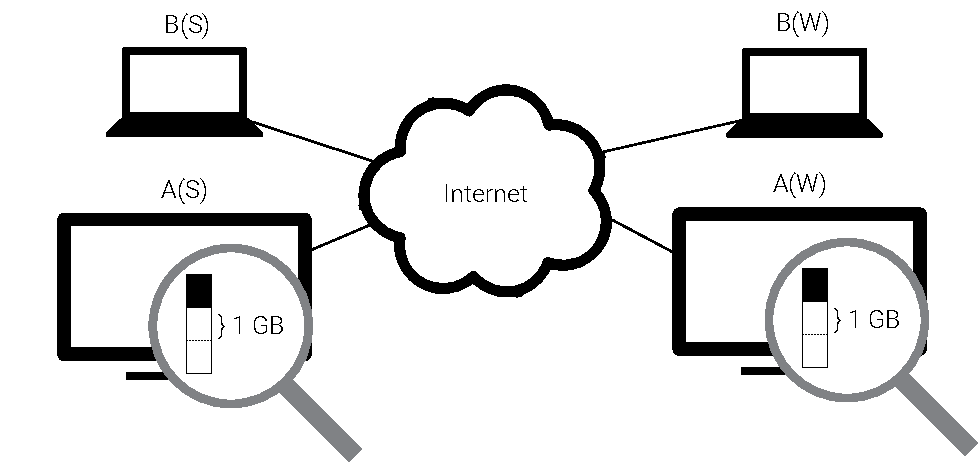
\includegraphics[]{images/partnerschaften_1.pdf}
	\label{partnerschaften_1}
  \caption{Wahl eines Geräts, auf dem Speicherplatz freigegeben wird.}
\end{figure}
Nun tauschen die Geräte A(S) und A(W) ihre Adressen aus und tragen sie beim jeweils anderen
in die Liste der Partnergeräte ein.
\begin{figure}[htb]
	\centering
  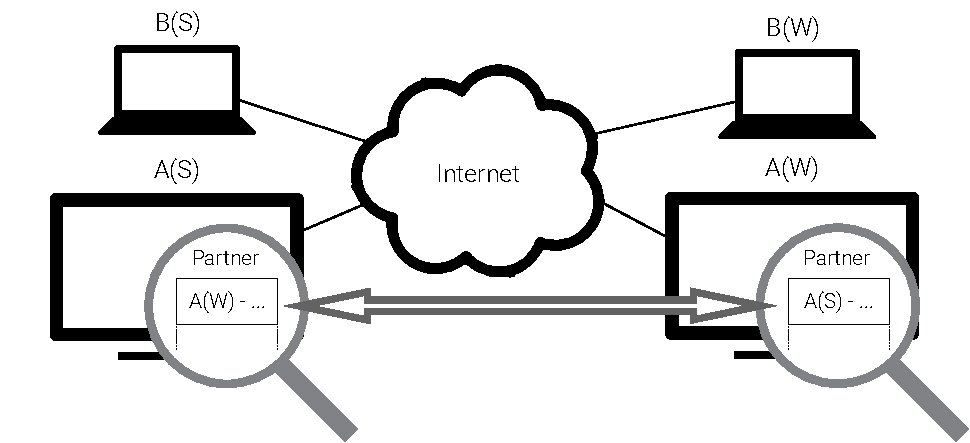
\includegraphics[]{images/partnerschaften_2.pdf}
	\label{partnerschaften_2}
  \caption{Austausch und Eintragen der Adressen.}
\end{figure}
Sobald beide Geräte gleichzeitig online sind, werden alle Geräte von Susanne auf Gerät A(W)
und umgekehrt alle Geräte von Wilfried auf Gerät A(S) gespeichert.
\begin{figure}[htb]
	\centering
  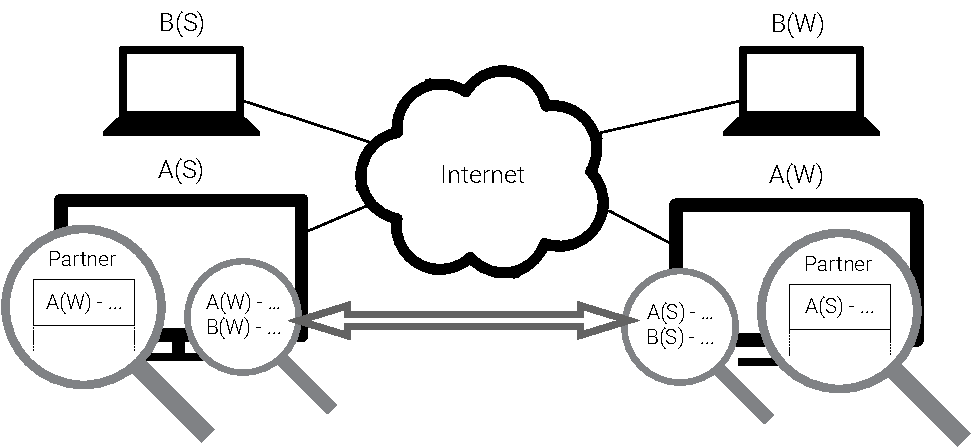
\includegraphics[]{images/partnerschaften_3.pdf}
	\label{partnerschaften_3}
  \caption{Eintragen der Geräte des Partners.}
\end{figure}
Weiters wird die Adresse von A(W) auf Susannes Geräte und die Adresse von A(S) auf Wilfrieds Geräte gespeichert.
\begin{figure}[htb]
	\centering
  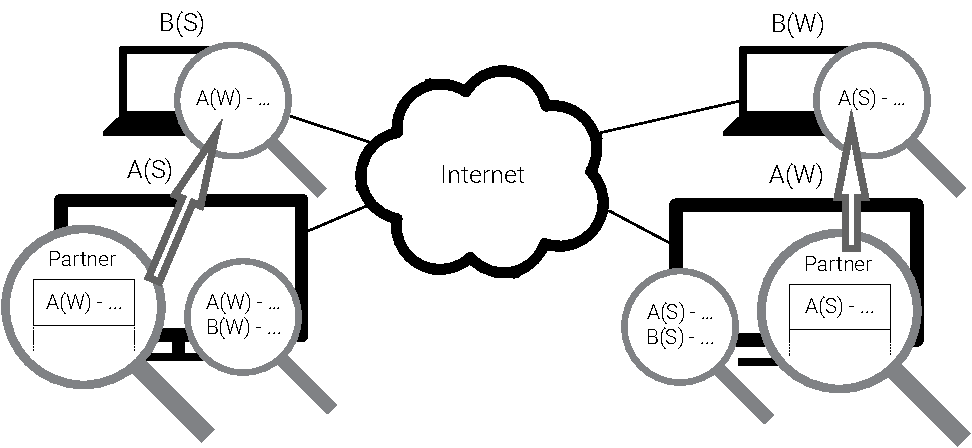
\includegraphics[]{images/partnerschaften_4.pdf}
	\label{partnerschaften_4}
  \caption{Eintragen der Adressen des Partnergeräts.}
\end{figure}
Ab diesem Zeitpunkt werden alle Änderungen von Susannes Dateien auf Gerät A(W) gesichert,
bis sie auf alle Geräte von Susanne verteilt wurden. Sobald Susannes Geräte die Änderung
erhalten, wird Gerät A(W) wieder aufgefordert, die Daten zu löschen. Das gleiche gilt natürlich
auch für Wilfried und das Gerät A(S).
